\documentclass{jsarticle}
\usepackage[dvipdfmx]{graphicx}
\begin{document}

\title{ライフゲームを作ろう}
\author{宇佐美雅紀}
\maketitle

Haskellの練習として、ライフゲームを作成します。

\section{ライフゲームとは}
ライフゲームは、生命の誕生、進化、淘汰などのプロセスを簡易的なモデルで再現したシミュレーションゲームであり、セル・オートマトンの一種です。
詳しくは、Wikipediaでライフゲームを検索してみてください。
\begin{verbatim}
( http://ja.wikipedia.org/wiki/%E3%83%A9%E3%82%A4%E3%83%95%E3%82%B2%E3%83%BC%E3%83%A0 )
\end{verbatim}

\section{ライフゲームのルール}

\begin{description}
 \item[誕生] 死んでいるセルに隣接する生きたセルがちょうど3つあれば、次の世代が誕生する。
 \item[生存] 生きているセルに隣接する生きたセルが2つか3つ以下ならば、次の世代でも生存する。
 \item[過疎] 生きているセルに隣接する生きたセルが1つ以下ならば、過疎により死滅する。
 \item[過密] 生きているセルに隣接する生きたセルが4つ以上ならば、過密により死滅する。
\end{description}

\begin{center}
 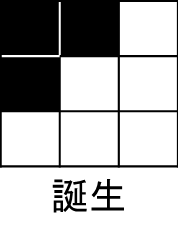
\includegraphics[width=2cm]{reproduction.png}
 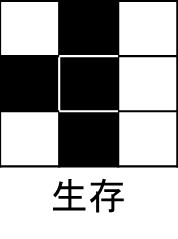
\includegraphics[width=2cm]{next-generation.png}
 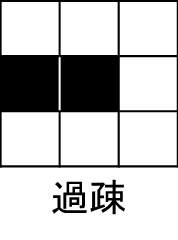
\includegraphics[width=2cm]{under-population.png}
 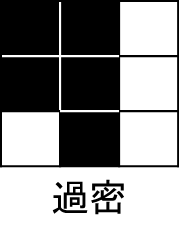
\includegraphics[width=2cm]{overcrowding.png}
\end{center}

\section{ライフゲームのデータ構造}
ライフゲームは任意のサイズ(NxM)の格子状のゲーム盤上で動作します。
ここでは、簡単のために格子のサイズは縦横同じとします(NxN)。
格子の各マスは、生きているか死んでいるかのどちらかです。

レコード構文を使って、以下のように定義します。
\begin{verbatim}
 data Lifegame = Lifegame { size :: Int
                           , board:: [(Int, Int)]
                           }
\end{verbatim}

boardはタプルのリストで、ゲーム盤上で生きているセルがいる場所を示します。
タプル(ダブル)はゲーム盤上の位置(x座標、y座標)を示します。
タプルが指示していない位置は、生きているセルがいません。

\begin{center}
 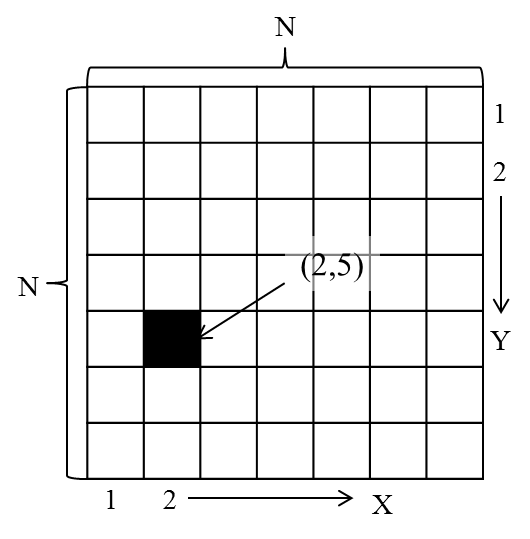
\includegraphics[width=4cm]{gameboard.png}
\end{center}

\section{ライフゲームの開発}
\subsection{ライフゲームの構造}

新しい世代を得る 
newGeneration :: Lifegame -> Lifegame
	現世代のゲーム盤を入力して、
	(1,1)~(size,size)のすべてのセルをチェックし
	生きているセルを見つけて
	新世代のゲーム盤を得る

指定セルが生きているかどうかをチェックする
isAlive :: (Int, Int) -> Lifegame -> Bool
	ゲーム盤上のセルの位置と、ゲーム盤を入力し
	指定されたセルが新世代で生きているかどうかをチェックする

指定セルの周囲の生きているセルの数を数える
countAlive :: (Int, Int) -> Lifegame -> Int
	ゲーム盤上のセルの位置と、ゲーム盤を入力し
	指定されたセルの周囲の生きているセルの数をカウントする


\subsection{ライフゲームの要素}
\subsubsection{指定セルの周囲の生きているセルの数を数える}
入力:ゲーム盤, 指定セル(x, y) 

出力:指定セルの周囲の生きているセルの数 : Int


\end{document}
